\documentclass[manuscript]{acmart}

\addtolength{\textfloatsep}{-10pt}

\copyrightyear{2021}
\acmYear{2021}
\setcopyright{rightsretained}
\acmConference[EMICS '21]{EMICS '21: ACM CHI '21 Workshop on Eye Movements as an Interface to Cognitive State}{May 14, 2021}{Yokohama, Japan}
\acmBooktitle{EMICS '21: ACM CHI '21 Workshop on Eye Movements as an Interface to Cognitive State, May 14, 2021, Yokohama, Japan}
\acmDOI{}
\acmISBN{}

\begin{document}

\title{Towards Robust Binary Communication Using Pupil Dilation by Mental Arithmetic}

\author{Immo Schuetz}
\orcid{https://orcid.org/0000-0002-3273-6237}
\email{immo.schuetz@psychol.uni-giessen.de}
\affiliation{
  \institution{Justus-Liebig University Giessen}
  \city{Giessen}
  \country{Germany}
 }
\affiliation{
  \institution{Chemnitz University of Technology}
  \city{Chemnitz}
  \country{Germany}
 }
 
\author{Julia Trojanek}
\email{julia.trojanek.jt@gmail.com}
\affiliation{
  \institution{Chemnitz University of Technology}
  \city{Chemnitz}
  \country{Germany}
 }

\author{Wolfgang Einhäuser}
\email{wolfgang.einhaeuser-treyer@physik.tu-chemnitz.de}
\affiliation{
  \institution{Chemnitz University of Technology}
  \city{Chemnitz}
  \country{Germany}
 }

\renewcommand{\shortauthors}{Schuetz, Trojanek \& Einhäuser}

\begin{abstract}
 The pupil reliably dilates with increases in cognitive load, e.g., when performing mental multiplication. This mechanism has previously been used for communication with Locked-In-Syndrome patients \cite{Stoll2013}, providing a proof-of-principle without focusing on communication speed. We investigated a similar paradigm in a larger sample of healthy participants (N=24) using three different eye trackers, including a sub-\$100 commercial solution. Using the previously suggested training-free approach, we reliably decoded binary (yes/no) responses with comparable performance in all devices. To address whether throughput can be increased without sacrificing accuracy, we explored different classification models. Using a support-vector machine (SVM), we reached useful decoding with as little as 5 s of data. Our results confirm that mental arithmetic-based pupil dilation is a viable communication solution and suggests that bitrates of high-end brain-computer interfaces (BCI) can be reached at substantially lower cost.
\end{abstract}

%%
%% The code below is generated by the tool at http://dl.acm.org/ccs.cfm.
%% Please copy and paste the code instead of the example below.
%%
\begin{CCSXML}
<ccs2012>
   <concept>
       <concept_id>10003120.10011738.10011775</concept_id>
       <concept_desc>Human-centered computing~Accessibility technologies</concept_desc>
       <concept_significance>500</concept_significance>
       </concept>
   <concept>
       <concept_id>10003120.10003121.10011748</concept_id>
       <concept_desc>Human-centered computing~Empirical studies in HCI</concept_desc>
       <concept_significance>500</concept_significance>
       </concept>
   <concept>
       <concept_id>10003120.10003121.10003128</concept_id>
       <concept_desc>Human-centered computing~Interaction techniques</concept_desc>
       <concept_significance>300</concept_significance>
       </concept>
 </ccs2012>
\end{CCSXML}

\ccsdesc[500]{Human-centered computing~Accessibility technologies}
\ccsdesc[500]{Human-centered computing~Empirical studies in HCI}
\ccsdesc[300]{Human-centered computing~Interaction techniques}

\keywords{pupil dilation, pupillometry, brain-computer interface, cognitive load, mental arithmetic}


\maketitle

\section{Introduction \& Related Work}

In patients whose motor capabilities are severely limited, such as Amyotrophic Lateral Sclerosis patients, the ocular and pupillary muscles often remain under volitional control even when the disease has progressed far. This makes eye tracking and pupillometry a potentially powerful method to provide a brain-computer interface (BCI) for communication \cite{majaranta2011gaze}. Unlike methods that operate directly on brain activity, like electroencephalography (EEG, e.g. \cite{Birbaumer1999}) or functional near infrared spectroscopy (fNIRS, e.g. \cite{borgheai2020enhancing}), eye tracking and pupillometry can be conducted with inexpensive off-the-shelf equipment and without direct contact to the user, allowing for a potentially wider range of use cases. Besides the well-known Pupillary Light Reflex (PLR), changes in pupil size reflect a multitude of task-related and cognitive influences (see \cite{Beatty2000,Einhauser2017,Mathot2018review} for reviews). Various approaches to achieve communication using volitional control of pupil size have been suggested. For example, modulations of the PLR by oscillatory changes in brightness can be used to decode one of multiple response alternatives simply by shifts of covert attention to an oscillating target \cite{Naber2013,Mathot2015,Mathot2016}. Pupil size modulation by mental imagery of a bright or dark scene \cite{Laeng2014} was explored for binary communication \cite{Diedrichs2015}, and the link between accommodation and pupil size ("near triad", e.g. \cite{Kasthurirangan2005}) was recently exploited in a similar way \cite{Ponzio2019}. Other recent work suggests that voluntary pupil control can be trained through biofeedback techniques based on affective mental imagery \cite{Ehlers2016,Ehlers2015,Ehlers2018training}, and this method has also shown promise as an input channel for HCI applications \cite{Strauch2017, Strauch2017a, Ehlers2018view}. Stoll and colleagues \cite{Stoll2013} proposed a communication method that exploits the robust and well-established relation between pupil dilation and cognitive load \cite{Hess1964,Beatty2000,Beatty1982,Kahneman1966}, specifically load induced by mental arithmetic, which has already been described at the end of the nineteenth century \cite{Heinrich1896,Ahern1979,Klingner2008,Chen2014}: Participants performed a mental multiplication task in one out of two separate time intervals, corresponding to either a "yes" or "no" response, and responses were successfully decoded from the difference in pupil dilation between both intervals. Importantly, this method required neither training on the task nor specific adjustments of the analysis to the individual and was successfully applied in locked-in-syndrome (LIS) patients. 
Since the goal of Stoll et al. (2013) \cite{Stoll2013} was a proof-of-principle that pupil-based communication is possible in this patient group, where communication at virtually any speed is beneficial, these authors were not concerned with optimizing throughput. While \cite{Stoll2013} clearly demonstrated the viability of the mental arithmetic paradigm for communication, it used a medical grade wearable eye tracker \cite{Stoll2011,Schneider2009} and tested a relatively small sample of N=6 healthy control participants, mostly to optimize their parameter settings for later use in patients. Using more affordable eye tracking hardware would enable easy accessibility and allow for broader clinical or in-home use of a pupil-based BCI. In the present study, we evaluate a similar task as \cite{Stoll2013} in a sample of N=24 healthy participants and compare the same medical eye tracker (EyeSeeCam) to a low-cost commercial (EyeTribe) as well as a research-grade device (Eyelink 1000+). Moreover, we compare different classification strategies to the method used in \cite{Stoll2013}, with the aim of improving decoding accuracy and communication throughput. 

\section{Mental Arithmetic Task}

\paragraph{Participants} A total of N=24 participants (10 female, 14 male; ages 20-33 years) took part in the study. Volunteers had normal or corrected-to-normal vision, no history of vision or neuromuscular disorders, provided written informed consent and were paid 6€/h for their participation.

\paragraph{Experimental Setup \& Paradigm} Participants performed a mental arithmetic task while their eye movements and pupil size were recorded using one of three eye trackers: Eyelink 1000+ (EL; SR-Research, Ottawa, ON, Canada) at 1000 Hz, EyeSeeCam Sci (ESC; EyeSeeTec GmbH, Munich, Germany; \cite{Stoll2011,Schneider2009}) at 220 Hz, and EyeTribe (ET; TheEyeTribe, Copenhagen, Denmark) at 60 Hz sample rate. The order of devices and sessions was counterbalanced across participants. Only one eye tracker was active at any given time to avoid interference from different IR illuminators. Participants placed their chin on a chin rest (distance to screen: 80 cm) and fixated a central cross during trials to keep effects of pupil foreshortening constant \cite{Hayes2016,Drewes2012}. A trial began with the presentation of one of seven binary questions on an LCD monitor until key press. Questions were chosen to have an objectively correct answer based on situative knowledge (e.g., "Is today Monday?") or information collected from the participant (e.g., "Is your name Michael?") and were always presented twice, once worded with "yes" as the correct response and once with "no" (14 trials per participant). After the key press, a  response (e.g., "yes") was presented for 10 s together with a multiplication task (first response interval, Fig. \ref{fig:pupil}, left), followed by the alternative response ("no") and a different multiplication for 10 s (second response interval). The order of questions (trials) and response alternatives within a trial were counterbalanced. Participants were instructed to perform the mental arithmetic task in the interval showing the correct response, and perform no task besides fixation in the other interval. 

\paragraph{Data Processing} The experiment was built in OpenSesame \cite{Mathot2012} and PyGaze \cite{Dalmaijer2014}. Custom PyGaze code was written to record data from the EyeSeeCam device.  Data from the left eye were analyzed, except for one participant where only data from the right eye were available and thus used. Eye blinks including 100 ms of data before and after the blink were removed and resulting gaps were linearly interpolated. Each experimental session was separately z-standardized (zero mean, unit standard deviation) to harmonize pupil size measures reported by different devices and match individual variation in baseline pupil size. All data were then resampled to a sample rate of 60 Hz using linear interpolation to match the slowest eye tracking device (ET)\footnote{To rule out low sampling rate as a major influence on classification, we repeated the same analyses with all data upsampled to 1 kHz to match Eyelink, with qualitatively similar results. Both analyses can be found on the project's Github page.}. Pupil traces of each trial and individual response interval were extracted relative to the onset of the first response interval, and subtractive baseline correction was applied based on the first second of data \cite{Mathot2018}. Pupil analyses were performed in Python (v. 3.7), ROC statistics in R (v. 4.0.3) with the pROC package \cite{Robin2011}. Uncorrected p-values are reported throughout, but all results that are given as significant at a 0.05 or 0.001 $\alpha$-level remain significant at this level after Bonferroni-Holm adjustment. Data and code are available online \footnote{\url{https://github.com/ischtz/emics2021-mentarith-bci}}.

\begin{figure}
    \centering
    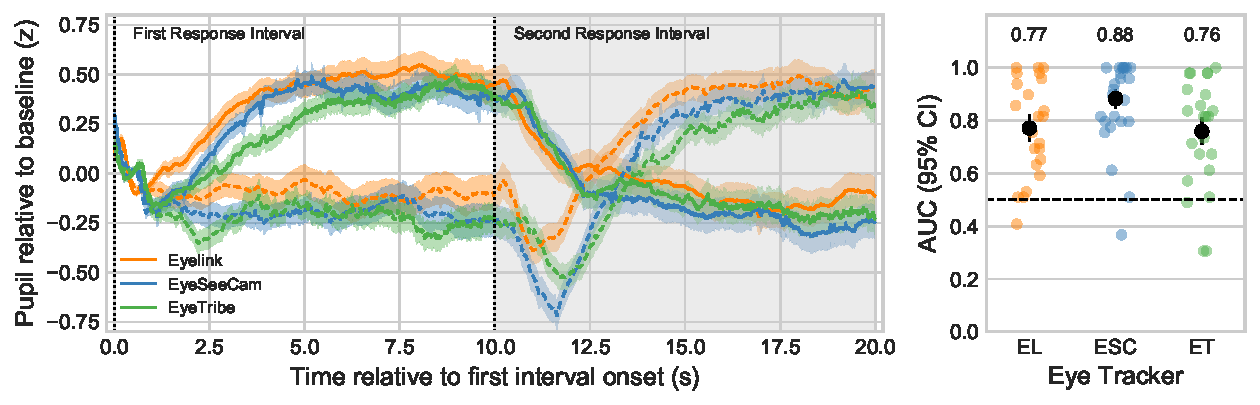
\includegraphics[width=1\textwidth]{figure1.pdf}
    \caption{\textit{Left}: Average pupil size change (z-scored; shading: $\pm$ 1 SEM) when participants performed mental arithmetic in the first (solid lines) and second (dashed lines) response interval. Dotted vertical lines indicate response period onsets. \textit{Right}: Small circles: Individual Area under the ROC curve (AUC) when decoding responses using the slope method used in \cite{Stoll2013}. Large circles and labels: AUC when decoding using all available responses for each device (using the method in \cite{Stoll2013}; error bars: 95\% CI, dashed line: chance level).}
    \label{fig:pupil}
\end{figure}

\section{Results}

\paragraph{Eye Tracker Comparison} As a first step, we replicated the analysis of \cite{Stoll2013} without any adjustment of parameters or fitting. We computed the receiver operator characteristic (ROC) curve for separating the interval containing the correct response option from the interval with the incorrect response option based on the slope from t=1.5s to t=5s of each interval. We quantified the sensitivity for discriminating the response options by the area under the ROC curve (AUC). To test statistically whether an individual's AUC exceeded chance (0.5) and to compare AUCs between devices, we used DeLong's test \cite{deLong1988, Robin2011}. Numerically, 23/24 (EL, ESC) or 21/24 (ET) participants had AUCs above chance, with 12 (EL), 13 (ET) and 19 (ESC) reaching significant above-chance decoding on an individual level (Fig. \ref{fig:pupil}, right). To compare the eye tracking devices, we first aggregated data across all participants and computed a single ROC curve per device (black circles in Fig. \ref{fig:pupil}). Decoding was significantly better for ESC (AUC = 0.88) than for the other two devices (EL: AUC = 0.77; z = 3.50; p < .001 and ET: AUC = 0.76; z = 3.90; p < .001), which were not significantly different from each other (z = 0.33; p = .738). Interestingly, decoding performance on the aggregate data was in the same range as the average over individual decoding performances, indicating high consistency across participants. 

\paragraph{Trial Decoding} We tested how well three standard classification algorithms (Logistic Regression, k-Nearest-Neighbor and SVM) could decode the correct response interval (first or second) in a trial. The aggregate data contained 336 (24$\times$14) trials $\times$ 1,200 pupil samples (10 s per response period at 60 Hz), and all 1,200 samples were included as model features. We used a nested cross-validation (CV) strategy, with a 7-fold outer CV to split trials into a training (288 trials) and test set (48), and an 8-fold inner CV (252/36) for hyperparameter tuning using grid search. We compared the best models to the difference slope (\textit{DS}, cf Fig. \ref{fig:class}) method as described in \cite{Stoll2013}. For a fairer comparison with the trial-based classifiers, we also calculated the DS measure using the full 20 s trial trace for slope fitting (\textit{DS/full}). Fig. \ref{fig:class} (circles) shows average CV performance for all models. Final models were then fit to all data using optimal hyperparameters (LogR: C = 0.0001; kNN: k = 50; SVM: C = 1, $\gamma$ = 0.0001, rbf kernel) and overall ROC curves and AUC were computed per device and compared to the approach in \cite{Stoll2013}. All classifiers showed better decoding than DS for EL and ET data (all z > 3.29, all p < .001), whereas differences were not significant in ESC after correction (all z < 2.44, all p > .015). DS/full was outperformed by all models on EL and ESC (all z > 3.73, all p < .001), but not on ET (all z < 2.60, all p > .001). SVM outperformed most models across devices significantly (all z > 2.93, all p < .001) except for DS on ESC (z = 2.43, p = .015), DS/full on ET (z = 2.60, p = .009) and kNN on ET (z = 1.97, p = .049) and EL (z = 0.07, p = .941). To investigate how decoding performance varied with data availability, we further evaluated the SVM model for pupil traces of varying length, starting at first interval onset and increasing in 250 ms steps (Fig. \ref{fig:class}, left) using 7-fold CV. Performance rapidly increased around 3 s after onset, then further improved when samples from the corresponding period of the second interval were included ($\geq$ 12.5 s). 

\begin{figure}
    \centering
    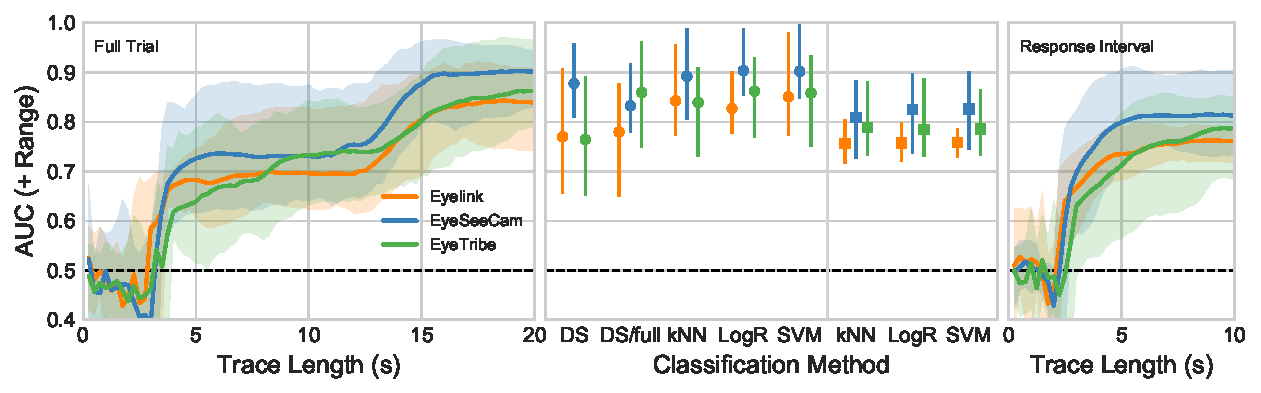
\includegraphics[width=1\textwidth]{figure2.pdf}
    \caption{Decoding Analysis. \textit{Left:} AUC of the best-performing SVM model when trained and tested on time windows in steps of 250 ms (7-fold CV). \textit{Middle:} Average cross-validation performance (AUC) of different algorithms in trial decoding (left; circles) and response interval decoding (right; squares). DS: Difference slope method - timing as in \cite{Stoll2013}; DS/full: DS method applied to full trial duration. \textit{Right:} Best model (SVM) AUC when trained and tested on separate response intervals, 250 ms intervals. Error bars / shading: AUC range in 7-fold CV. Black dashed line: chance level.}
    \label{fig:class}
\end{figure}

\paragraph{Interval Decoding} We further explored task decoding of individual response intervals (calculate or rest) using pupil data from the individual 10 s response intervals (two intervals per trial; 672 intervals $\times$ 1,200 pupil samples in total). Models and CV strategy were identical to trial decoding. On this dataset, performance was lower than with full trials but still well above chance (Fig. \ref{fig:class}, squares). SVM and kNN achieved comparable performance (all z < 2.36, p > .018), generally better than LogR (all z > 3.20, p < .002 except kNN/EL: z = 1.33, p = .182). As with trial traces, we selected SVM for follow-up trace length analysis (Fig. \ref{fig:class}, right). Performance again steeply increased after the first 2.5 s of data, reaching asymptotic performance after 5 s.  

\section{Discussion}
We demonstrate that robust communication by controlling one's pupil through mental arithmetic can be achieved with a variety of devices, including a sub-\$100 eye tracker. With a larger set of healthy users, we replicated that the method suggested by Stoll and colleagues \cite{Stoll2013} achieves good performance, in particular for the head-mounted device (ESC) also used in their study. Nonetheless, supervised learning methods further improve classification performance. Our data suggest that a single 5-s response interval (calculate or rest) would be sufficient for decoding, allowing an at least four-fold speed up compared to \cite{Stoll2013}. It is conceiveable that decoding can be further improved in patients and healthy users by applying time series-aware models, continuous cognitive load measures such as the Index of Cognitive Activity (ICA, \cite{Marshall2002ICA}) and (Low/High-) Index of Pupillary Activity (IPA / LHIPA, \cite{Duchowski2018,Duchowski2020}), or neural network models, provided sufficient data are available. Importantly, our method does not require any adjustment to the individual user (aggregate data was used), though further improvements may be possible if more trials per user are recorded and classifiers are trained on an individual level. While the EyeTribe device used here is no longer available commercially, the results presented are based on a sampling rate of 60 Hz and are likely to generalize to similar low-end devices. Additionally, robust pupillometry based on webcam or smart phone camera data is now within reach (e.g., \cite{wangwiwattana2018pupilnet, mazziotti2021meye}), which could further expand the possible fields of application for HCI approaches that exploit volitional pupil control based on mental arithmetic.

\bibliographystyle{ACM-Reference-Format}
\bibliography{literature}

\end{document}
\endinput

